\begin{frame}[label=gnss_viability]
    \frametitle{TOF Precision depends on \alert{Measurement Errors}}
    % \textit{Position estimate uncertainties depends on...}  (1) \colorbox{yellow}{\textbf{Measurement Errors}}
    \begin{columns}[T]
        \begin{column}{0.5\textwidth}
            Range measurements have uncertainty: %
            \begin{center}
                \(\sigma_\rho = \sqrt{2\sigma^2_{clk} + 2\sigma^2_{pos} + \sigma^2_{\Delta\tau}}\)
            \end{center} %
            {\setlength{\leftmargini}{1em} \begin{itemize}
                \item \(\sigma_{clk} = \qty{3}{\m}\): \textcolor{blue}{\textbf{TX}}/\textcolor{red}{\textbf{RX}} clock instability
                \item \(\sigma_{pos} = \qty{1}{m}\): \textcolor{blue}{\textbf{TX}}/\textcolor{red}{\textbf{RX}} positional uncertainty
                \item \(\sigma_{\Delta\tau} \approx \sqrt{\frac{1}{2 T_{coh} C/N_0}} \): Signal correlation error
                \begin{itemize}
                    \item 8 m typical 
                    \item \(T_{coh}\): Coherent integration time
                    \item \(C/N_0\): Carrier-to-noise ratio
                \end{itemize}
            \end{itemize}}
        \end{column}
        \vrule{}
        \begin{column}{0.5\textwidth}
            \alert{Correlation error}: Meteor trail is \textit{\textbf{not}} a point-like reflector
            \begin{itemize}
                \item Elongated reflector smears echo
                \item Correlation against \textcolor{blue}{\textbf{TX}} waveform \(\xrightarrow[]{}\) positive range bias (\textcolor{green}{\textit{\textbf{green}}})
            \end{itemize}
            \centering
            \begin{tikzpicture}
                    \node[anchor=east, inner sep = 0] (img1) at (0,0) { 
                        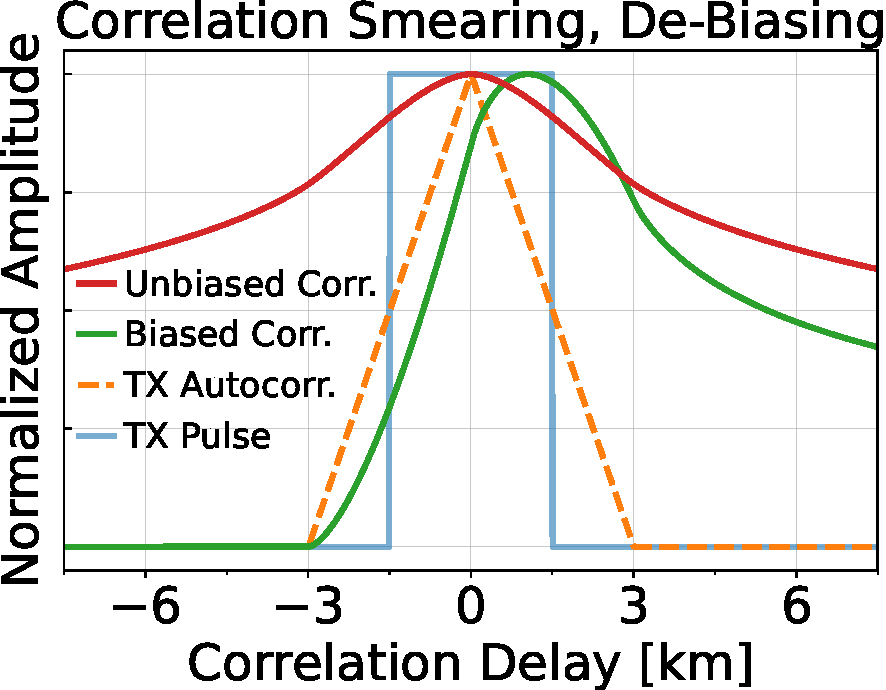
\includegraphics[width=0.55\linewidth]{img/corr_smear_0F1.pdf}
                    };
                    \node[anchor=west, inner sep=0] (img) at (img1.east) {%
                        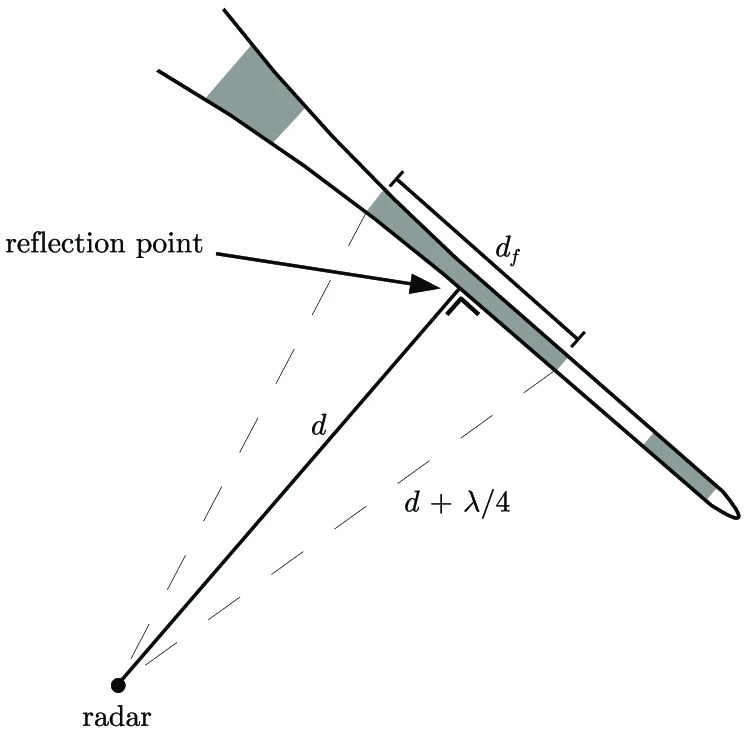
\includegraphics[width=0.4\linewidth]{img/verbeeck_ProceedingsRadioMeteor_2005.png}
                    };
                    \node[anchor=north east, inner sep=2pt] at ([yshift=-0.0cm]img.north east) { 
                    {{{\fontsize{3}{3.4}\selectfont\raggedleft \textcolor{black}{\textit{Credit:} \citeauthor{verbeeck_ProceedingsRadioMeteor_2005}, \citeyear{verbeeck_ProceedingsRadioMeteor_2005} \cite{verbeeck_ProceedingsRadioMeteor_2005}}}}}
                };
            \end{tikzpicture}
        \end{column}
    \end{columns}
    \centering % 
    \alert{De-biased Trail correlation function derived} (\textcolor{red}{\textit{\textbf{red}}})
\end{frame}

\begin{frame}[label=precision_requirements]
    \frametitle{TOF Precision: Propagation and Requirements}
    \begin{columns}
        \begin{column}{0.7\textwidth}
            TOF precision depends on \alert{array geometry}: 
            \begin{center}
                \scriptsize
                \alert{Larger array} \(\xrightarrow[]{}\) More diverse measurements
                
                \(\xrightarrow[]{}\) \alert{smaller positional uncertainties}
            \end{center}

            Quantified through dilution of precision (DOP) matrix: 
            {\scriptsize \begin{equation*} \scriptsize
                \mathbf{H} = \left( \mathbf{G}^{\top} \mathbf{G} \right)^{-1}
            \end{equation*}}
            %
            {Measurement \alert{errors are propagated} to get positional uncertainties: 
            {\scriptsize 
            \begin{align*}
                \begin{matrix}  
                    \sigma_E = \sigma_{\rho} \cdot \sqrt{H_{1,1}}  \qquad \qquad & \sigma_N = \sigma_{\rho} \cdot \sqrt{H_{2,2}} & \qquad \qquad \sigma_U = \sigma_{\rho} \cdot \sqrt{H_{3,3}} 
                \end{matrix}
            \end{align*}}}

            
                \begin{tcolorbox}[width=\linewidth, halign=center,  boxrule=1pt, arc=0pt,auto outer arc,left=0pt,right=0pt,boxsep=0pt]
                Science-driven positional precision requirement:

                \hl{\textbf{1 km uncertainty in altitude}}
            \end{tcolorbox}
        \end{column}
        \begin{column}{0.3\textwidth}
            \begin{tikzpicture}
                \node[anchor=center, inner sep=0] (img) at (0,0) {
                    {{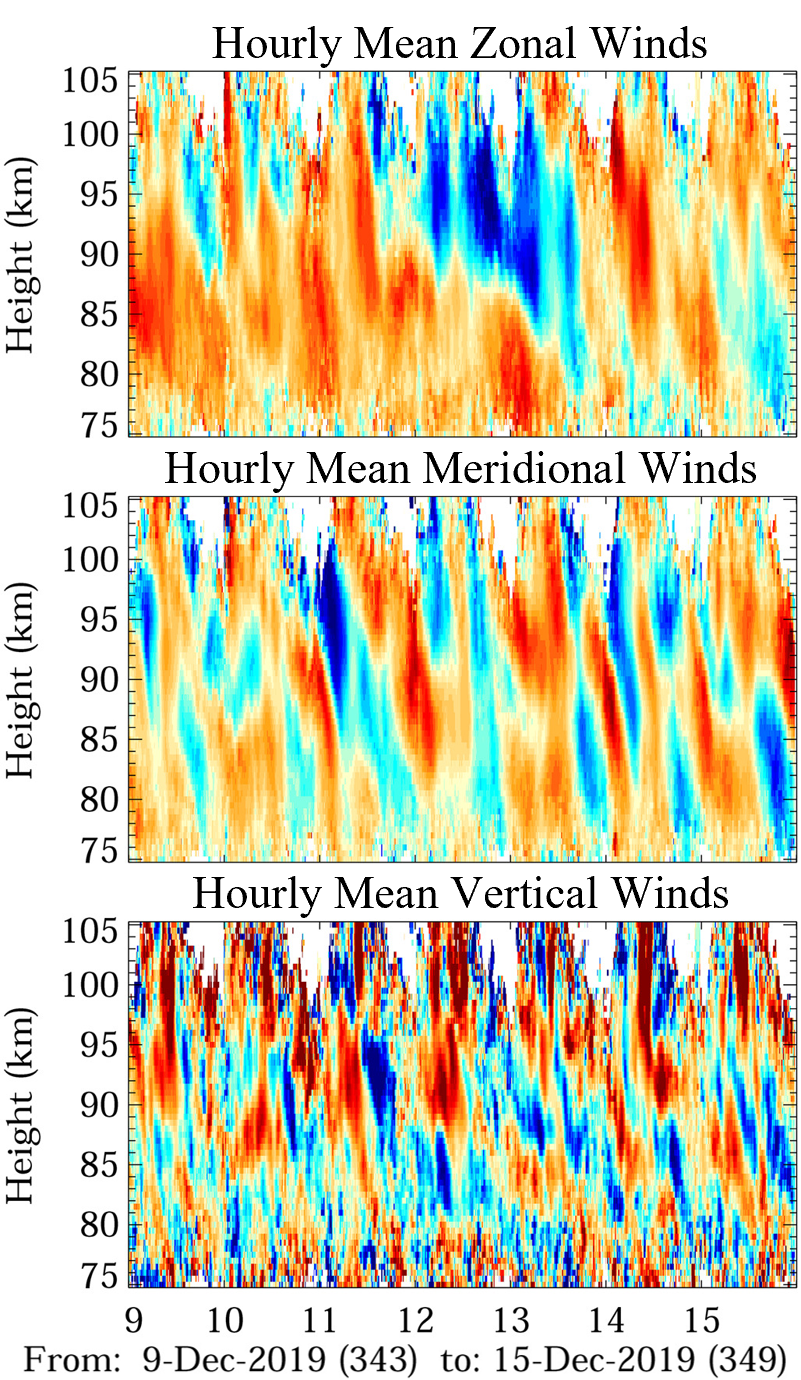
\includegraphics[width=0.7\linewidth]{img/chau_MultistaticSpecularMeteor_2021.png}}}
                };
                \node[anchor=east, inner sep=2pt] at ([yshift=-0.2cm]img.east) { 
                    {{{\fontsize{3}{3.4}\selectfont\raggedleft \textcolor{black}{\textit{Credit:} \citeauthor{chau_MultistaticSpecularMeteor_2021}, \citeyear{chau_MultistaticSpecularMeteor_2021} \cite{chau_MultistaticSpecularMeteor_2021}}}}}
                };
            \end{tikzpicture}        
            {\setlength{\leftmargini}{1em} \begin{itemize} \scriptsize
                \item 2 km altitude bins common
                \item Vertical wavelength of studied dynamics: \(\sim\)10s of km
            \end{itemize}}  
        \end{column}
    \end{columns}
\end{frame}

